\providecommand{\isolatedBuild}[1]{#1}% fallback definition lets this file build normally
\isolatedBuild
{
\documentclass[11pt,letterpaper]{book}
\usepackage{import}

% This file must be found via the TEXINPUTS environment variable.
%\documentclass[11pt,letterpaper]{book}

% aleeper: I think these are needed for Paul's macros?
\usepackage{epsfig}
\usepackage{epstopdf}

%\makeatletter
%\typeout{The import path is \import@path}
%\makeatother

\usepackage{import}

\subimport{./}{packagesMitiguy.sty}
\subimport{./}{macrosMitiguy.tex}
\subimport{./}{PageStylesMitiguy.tex}
\subimport{./}{macrosLeeper.tex}


\pagestyle{plain}
\pagenumbering{arabic}

\begin{document}
\HandoutHeader{ENGR 14 - Vector Geometry Examples}
%
\vspace{-0.5pc}
\small
%
\textColorBold{darkerBlue}{Vector Geometry - Distance}
\\[0.45pc]
}
%%%%%%%%%%%%%%%%%%%%%%%%%%%%%%%%%%%%%%%%%%%%%%%%%
%
Imagine you are installing a zip-line from the \textbf{top} of the south tower
of the Golden Gate Bridge (point `B') to the dock at Torpedo Wharf (`A').
\\[0.45pc]
%
\begin{minipage}[t]{0.5\linewidth}
%
A convenient coordinate system to set up for your analysis is
\uvecx{n} pointing east (right on the map), \uvecy{n} pointing north (up on the map),
and \uvecz{n} pointing ``up'' (away from the ground).
You may \textbf{assume} these unit vectors are orthogonal to each other.
%
\\[0.5pc] You may assume the dock is at height 0 m.
%
\\[0.5pc]
{\footnotesize
\begin{tabular}{|l|c|r|}
           \hline Quantity                      & Symbol     & Value      % & (Initial) Value(s)
  \\[0.0pc]\hline
 	        Height of bridge tower              & $h$        & 67 m  % & \valueUnits{0}{deg}
  \\[0.0pc] East-West distance from A to B      & $x$        & 711 m  % &
  \\[0.0pc] North-South distance from A to B    & $y$        & 538 m  % & \valueUnits{200}{kg}
  \\[0.0pc]\hline
\end{tabular}}
\end{minipage}
\hfill
\begin{minipage}[t]{0.5\linewidth}
\vspace*{-0.5pc}
\flushright
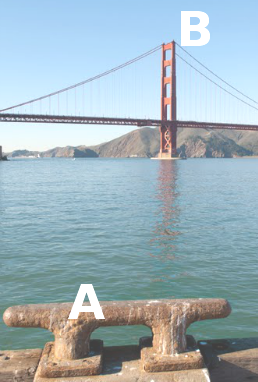
\includegraphics[height=5cm]{bridge.png}
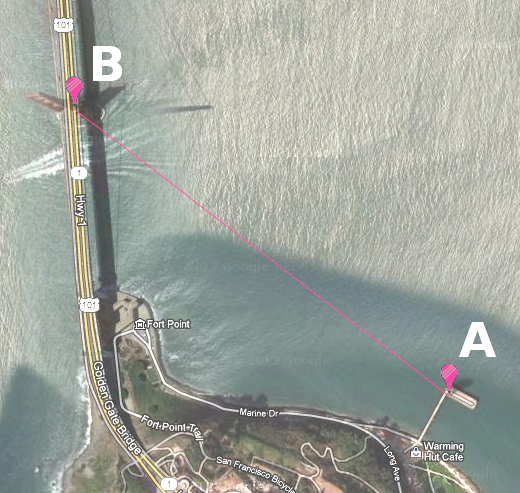
\includegraphics[height=5cm]{map2.png}
\end{minipage}

\begin{enumerate}
\item Sketch the \uvecBasisxyz{n} unit vectors on the map above.
\\[-0.5pc]
\item Write the position vector to B from A: \hspace{0.5cm}
\posvec{A}{B} = \rule{2cm}{0.2mm}~\uvecx{n} + \rule{2cm}{0.2mm}~\uvecy{n} + \rule{2cm}{0.2mm}~\uvecz{n}
\\[-0.5pc]
\item Use \posvec{A}{B} to estimate the minimum \textbf{length} of cable needed to span between A and B.
\vspace{12cm}

\item (Circle one.) The method \textbf{you} used in part (c) is
\begin{tabular}[t]{l}
(1) a special-case formula, or
\\[0.2pc]
(2) a general approach for any vector dot product.
\end{tabular}
\end{enumerate}

\isolatedBuild {
\vfill
\end{document} }

